%% LyX 2.2.2 created this file.  For more info, see http://www.lyx.org/.
%% Do not edit unless you really know what you are doing.
\documentclass{article}
\usepackage[T1]{fontenc}
\usepackage[latin9]{inputenc}
\usepackage{url}
\usepackage{amsmath}
\usepackage{graphicx}

\makeatletter

%%%%%%%%%%%%%%%%%%%%%%%%%%%%%% LyX specific LaTeX commands.
%% Because html converters don't know tabularnewline
\providecommand{\tabularnewline}{\\}

%%%%%%%%%%%%%%%%%%%%%%%%%%%%%% Textclass specific LaTeX commands.
\newenvironment{lyxcode}
{\par\begin{list}{}{
\setlength{\rightmargin}{\leftmargin}
\setlength{\listparindent}{0pt}% needed for AMS classes
\raggedright
\setlength{\itemsep}{0pt}
\setlength{\parsep}{0pt}
\normalfont\ttfamily}%
 \item[]}
{\end{list}}

\makeatother

\usepackage{listings}
\renewcommand{\lstlistingname}{Listing}

\begin{document}

\title{GenConstraint: A programming tool for constraint optimization problems}

\author{Ioannis G. Tsoulos$^{(1)}$\thanks{Corresponding author. Email: itsoulos@teiep.gr},
Vasileios Stavrou$^{(2)}$, Nikolaos E. Mastorakis$^{(2)}$, \\
Dimitrios Tsalikakis$^{(3)}$}

\date{$^{(1)}$Department of Informatics and Telecommunications, University
of Ioannina, Greece\\
$^{(2)}$Hellenic Naval Academy, Department of Computer Science, Military
Institutions of University Education, 18539 Piraeus, Greece,\\
$^{(3)}$University of Western Macedonia, Department of Engineering
Informatics and Telecommunications, Greece }
\maketitle
\begin{abstract}
This article presents a software used to solve constrained optimization
problems with a modified genetic algorithm. The software is written
entirely in ANSI-C++ and the user can prepare the objective function
either in C++ or in Fortran. The article presents the genetic algorithm,
the incorporated software as well as some experiments on a series
of optimization problems. Also, the proposed software was tested on
the design of a two-dimensional filter. The results are compared against
the results from the algorithm DONLP2.
\end{abstract}

\section{Introduction }

The constraint optimization problem can be formulated as 
\begin{eqnarray}
\min_{x} & f(x) & \mbox{subject to}\nonumber \\
 & g_{i}(x)\le0 & \ i=1,\ldots,m\nonumber \\
 & h_{j}(x)=0 & \ j=1,\ldots,p\label{eq:eq1}
\end{eqnarray}
where $x_{i}\in\left[a_{i},b_{i}\right],\ i=1,\ldots,n$. Many problems
from areas such as physics\cite{Physics1,Physics2}, engineering\cite{Eng1,Eng2},
medicine\cite{Med1,Med2}, economics\cite{Econ1} etc can be formulated
as constrained optimization problems and hence there is a great demand
for methods and software to tackle this problem. During the past years
many methods have been proposed for this problem, such as techniques
based on genetic algorithms\cite{Genetic1,Genetic2,Genetic3}, Particle
Swarm Optimization\cite{pso1,pso2,pso3}, Ant Colony Optimization\cite{aco1,aco2}
or even methods that utilize Artificial Neural Networks\cite{ann1}.
Also many software packages have been developed for solving constraint
optimization problems such as: PyOpt a Python based Object-Oriented
Framework for Nonlinear Constrained Optimization\cite{pyopt}, the
Grey Wolf Optimizer(GWO) algorithm\cite{wolf} which mimics the leadership
hierarchy and hunting mechanism of grey wolves in nature etc.

The proposed software presents and uses a modified version of the
genetic algorithm introduced in \cite{Tsoulos} for solving constrained
optimization problems. The original method has been enhanced by using
a periodical application of a global search procedure which preserves
the feasibility of the chromosomes.

The rest of this article has as follows: in section \ref{sec:Method-description}
a detailed description of the modified genetic algorithm is given,
in section \ref{sec:Description-of-software} the proposed software
is described in detail, in section \ref{sec:Experiments} the results
from a series of experiments with a variety of constrained optimization
problems are outlined and finally in section \ref{sec:Conclusions}
some conclusions and some guidelines for future research are presented.

\section{Method description \label{sec:Method-description}}

\subsection{The proposed algorithm }

The algorithm uses a population of chromosomes to solve the constraint
optimization problem. Every member of the population is a trial solution
expressed as a vector of $n$ double numbers. The proposed algorithm
has the following steps:
\begin{enumerate}
\item \textbf{Initialization step}.
\begin{enumerate}
\item \textbf{Set} the maximum number of generations ITERMAX.
\item \textbf{Set} the number of chromosomes K.
\item \textbf{Set} the selection rate $p_{c}$
\item \textbf{Set} the mutation rate $p_{m}$
\item \textbf{Set} the number of chromosomes for the global search procedure
$g_{c}$
\item \textbf{Set} the number of iterations for the global search procedure
$g_{I}$
\item \textbf{Initialize} the chromosomes as random vectors in the range
$[a,b]$.
\item \textbf{Set} iter=0
\end{enumerate}
\item \textbf{Evaluation step}. \label{enu:Evaluation-step.}
\begin{enumerate}
\item \textbf{For} every chromosome $C$ calculate the fitness of $C$.
The calculation of the fitness is outlined in subsection \ref{subsec:Fitness-calculation}.
\end{enumerate}
\item \textbf{Application} of genetic operators.

\begin{enumerate}
\item \textbf{Selection procedure}: The chromosomes are sorted in descending
order according to their fitness value. The first $\left(1-p_{s}\right)\times K$
chromosomes are transferred to the next generation. The rest of the
chromosomes are substituted by offsprings created through the crossover
procedure given in \cite{Tsoulos}.
\item \textbf{Mutation procedure: }perform mutation to the population with
mutation probability $p_{m}$
\item \textbf{Replace} the $p_{s}\times K$ worst chromosomes in the population
with the offsprings created by the genetic operators.
\end{enumerate}
\item \textbf{Set} iter=iter+1
\item If iter MOD $g_{I}$=0, then 
\begin{enumerate}
\item \textbf{Apply} the global search procedure, that described in subsection
\ref{subsec:The-global-search}.
\item \textbf{Apply} the local search procedure Cobyla \cite{cobyla} to
the best chromosome of the population.
\end{enumerate}
\item \textbf{Check} for termination. If the termination criteria met then
\textbf{goto} step \ref{enu:Local-search-step.}, else \textbf{goto}
step \ref{enu:Evaluation-step.} The termination criteria has as follows:
\begin{enumerate}
\item \textbf{Calculate} the variance $\sigma^{(\mbox{iter})}$ of the best
discovered value. 
\item The genetic algorithm terminates when 
\begin{equation}
\ \sigma^{(\mbox{iter})}\le\frac{\sigma^{(\mbox{last})}}{2}\mbox{\ \ \ OR iter>ITERMAX }\label{eq:termination_mine}
\end{equation}
 where last is the generation where the current best value was discovered
for the first time.
\end{enumerate}
\item \textbf{Local search step}.\label{enu:Local-search-step.} Apply the
local search procedure Cobyla to the best chromosome of the population.
\end{enumerate}

\subsection{Fitness calculation \label{subsec:Fitness-calculation}}

The calculation of the fitness is performed using with the application
of penalties in order to force the constraints to be satisfied. For
any chromosome $x$ are the following steps are taken place:
\begin{enumerate}
\item Estimate the objective function at $x$ using: 
\begin{equation}
v_{1}(x)=f(x)\label{eq:eq3}
\end{equation}
\item Compute the associate penalties for the equality constraints $h_{i}(x),\ i=1,..,p$
of the equation \ref{eq:eq1} as:
\begin{equation}
v_{2}(x)=\sum_{i=1}^{p}h_{i}^{2}(x)\label{eq:eq4}
\end{equation}
and accordingly for the inequality constraints $g_{i}(x),\ i=1,...,m$
\begin{equation}
v_{3}(x)=\sum_{i=1}^{m}G_{i}^{2}\left(g_{i}(x)\right)\label{eq:eq5}
\end{equation}
where the function $G(x)$ is defined as follows:
\begin{equation}
G(x)=\begin{cases}
0, & x\le0\\
x, & x>0
\end{cases}\label{eq:eq2}
\end{equation}
\item The fitness value is computed with:
\begin{equation}
v(x)=v_{1}(x)+\lambda v_{2}(x)+\lambda v_{3}(x)\label{eq:fitness}
\end{equation}
where $\lambda>0$.
\end{enumerate}

\subsection{The global search procedure \label{subsec:The-global-search}}

The global search procedure is used to enhance the fitness of some
chromosomes by exchanging genomes with other randomly selected chromosomes.
The procedure is the following:

\textbf{Select} randomly $g_{c}$ chromosomes from the genetic population
and create the set $L_{S}$ from these chromosomes
\begin{enumerate}
\item \textbf{For} every chromosome $X_{i}$ \textbf{in} $L_{S}$ 

\begin{enumerate}
\item \textbf{Select} randomly another chromosome $Y$ from the population
\begin{enumerate}
\item \textbf{If }$X_{i}$ is feasible and $Y$\textbf{ }is not feasible
\textbf{then} discard $Y$ \textbf{else }
\begin{enumerate}
\item \textbf{Create} an offspring of $X_{i}$ and $Y$ using one point
crossover. Denote the offspring as $Z$
\item \textbf{Obtain} the fitness $f(Z)$ of chromosome $Z$\textbf{. If}
$f(z)<f_{i}$ then $X_{i}=Z,\ f_{i}=f(Z)$
\end{enumerate}
\end{enumerate}
\item \textbf{Endif}
\end{enumerate}
\end{enumerate}

\section{Description of the software \label{sec:Description-of-software}}

\subsection{Installation }

The software can be downloaded from the relevant url: \url{http://itsoulos.teiep.gr/GenConstraint.tar.gz}
The software has been written in Ansi C++ for Unix based environments
and under any Unix system the user can issue the following commands
to compile and install the software.
\begin{enumerate}
\item gunzip GenConstraint.tar.gz
\item tar xfv GenConstraint.tar. After this command the directory \emph{GenConstraint}
will be created.
\item cd GenConstraint
\item Open with an editor the file \emph{Makefile.inc}. The contents of
the file are displayed in Figure \ref{fig:makefileinc}. In most cases,
the user should change only the last variable ROOTDIR in order and
he should setup the variable to refer to the current installation
directory.
\item Issue the command make.
\item The final outcome of the compilation is the command line utility \emph{make\_program}
located under the \emph{bin} subdirectory.
\end{enumerate}

\subsection{The utility make\_program}

The utility make\_program is used to produce the executable for the
objective function. The make\_program has the following command line
options:
\begin{enumerate}
\item \textbf{-h} Displays a help screen and the program terminates.
\item -\textbf{p} \emph{filename}. The parameter filename specifies the
name of the file with the objective function. The function could be
written either in C++ or in Fortran. In subsection a detailed description
of the formulation of the objective function is provided.
\item -\textbf{o} \emph{filename}. The output of the compilation is the
argument \emph{filename}. The parameter \emph{filename} is optional
and the default name used will be \emph{constraint}.
\end{enumerate}

\subsection{Problem formulation \label{subsec:Problem-formulation}}

An example of coding the objective problem in ANSI C++ is presented
in Figure \ref{fig:Coding-the-chootinan1} for the problem of chootinan1.
The following functions were used:
\begin{enumerate}
\item \textbf{int} getdimension(): This function returns the dimension of
the objective problem.
\item \textbf{int} geteq(): This function returns the number of equatlity
constraints.
\item \textbf{int} getineq(): This function returns the number of inequality
constraints.
\item \textbf{void} getleftmargin(\textbf{double} {*}x): This function returns
in the array x the lower bound for the objective problem. 
\item \textbf{void} getrightmargin(\textbf{double} {*}x): This function
returns in the array x the upper bound for the objective problem.
\item \textbf{double} funmin(\textbf{double} {*}x): This function returns
the objective function evaluated at the point x.
\item \textbf{void} feq(\textbf{double} {*}x,\textbf{double} {*}eq): This
function returns the equality constraints in the array eq evaluated
at the point x.
\item \textbf{void} fineq(\textbf{double} {*}x,\textbf{double} {*}ineq):
This function returns the inequality constraints in the array ineq
evaluated at the point x.
\item \textbf{void} done(\textbf{double} {*}x). The method done will be
called after the termination of the genetic algorithm. The parameter
x is the best value discovered by the genetic algorithm.
\end{enumerate}

\subsection{Compilation of the problem }

The utility\emph{ make\_program} is used to compile the objective
function and produce the final executable. For example in order to
compile the objective function \emph{salkin.cc} located under \emph{examples}
subdirectory the user should issue the following command:
\begin{lyxcode}
../bin/make\_program~-p~\emph{salkin.cc}
\end{lyxcode}

\subsection{Command line options}

The executable \emph{constraint} has a variety of command line options
as follows:
\begin{enumerate}
\item -h. Displays a help screen and terminates. 
\item -c \emph{count}. The integer parameter \emph{count} determines the
number of chromosomes for the genetic population. The default value
is 200.
\item -m \emph{value}. The float parameter \emph{value} determines the mutation
rate used in the genetic population. The default value is 0.05
\item -s \emph{value}. The float parameter \emph{value} determines the selection
rate used in the genetic population. The default value is 0.10
\item -p \{0|1\}. Specify the print level (0 or 1, default 1). If this parameter
has the value 1, then a detailed output of the progress of the genetic
algorithm will be printer, otherwise only the located global minimum
will be printed. 
\item -r \emph{seed}. The integer parameter \emph{seed} determines the seed
used for the random number generator. The default value is 1.
\item -d \emph{count}. The integer parameter \emph{count} specifies the
number of chromosomes used in the global search procedure. The default
value is 20.
\item -n \emph{generations}. The integer parameter \emph{generations} determines
the number of generations that after them the global search procedure
will take place. The default value is 20.
\item -g \emph{generations}. The integer parameter \emph{generations} sets
the maximum number of generations for the genetic algorithm.
\end{enumerate}

\section{Experiments \label{sec:Experiments}}

\subsection{A typical run}

Let us consider the problem Chootinan1. The problem is coded using
C++ and the corresponding file is the \emph{chootinan1.cc} located
under the \emph{examples} subdirectory of the distribution. The following
steps are required to apply the proposed method on this function:
\begin{enumerate}
\item cd examples
\item ../bin/make\_program -p chootinan1.cc
\item ./constraint
\end{enumerate}
The \emph{constraint} executable prints a series of lines to the terminal.
The last ten lines from an example run are listed below:

\begin{lstlisting}
GENERATION: 195	VALUE=            -15	FEASIBLE=YES  
GENERATION: 196	VALUE=            -15	FEASIBLE=YES  
GENERATION: 197	VALUE=            -15	FEASIBLE=YES  
GENERATION: 198	VALUE=            -15	FEASIBLE=YES  
GENERATION: 199	VALUE=            -15	FEASIBLE=YES  
GENERATION: 200	VALUE=            -15	FEASIBLE=YES  
GENERATION: 201	VALUE=            -15	FEASIBLE=YES 
1.000000 1.000000 1.000000 1.000000 0.999997 1.000000 1.000000 
    1.000000 1.000000 2.999990 3.000005 3.000005 1.000000  (      -14.9999962639) 
TOTAL FUNCTION CALLS =   102406 
\end{lstlisting}

The software prints in every line: Generation number, current global
minimum and the feasibility of the located minimum. At the end the
software prints the located global minimum as well as the total number
of function calls.

\subsection{Benchmark functions }

\subsubsection*{Levy problem}

This problem is described in \cite{levy} and it is given by: 
\[
\min_{x}f(x)=-x_{1}-x_{2}
\]
with $x\in[0,1]^{2}$, subject to 
\[
g_{1}(x)=\left\lfloor \left(x_{1}-1\right)^{2}+\left(x_{2}-1\right)\right\rfloor \left(\frac{1}{2a^{2}}-\frac{1}{2b^{2}}\right)+\left(x_{1}-1\right)\left(x_{2}-1\right)\left(\frac{1}{a^{2}}-\frac{1}{b^{2}}\right)-1\ge0
\]
with $a=2,\ b=0.25$. The value of global minimum is $f_{\mbox{min}}=-1.8729$.

\subsubsection*{Hess Problem}

This problem is described in \cite{Hess} and it is given by:
\[
\max_{x}f(x)=25\left(x_{1}-2\right)^{2}+\left(x_{2}-2\right)^{2}+\left(x_{3}-1\right)^{2}+\left(x_{4}-4\right)^{2}+\left(x_{5}-1\right)^{2}+\left(x_{6}-4\right)^{2}
\]
with $0\le x_{1}\le5,\ 0\le x_{2}\le1,\ 1\le x_{3}\le5,\ 0\le x_{4}\le6,\ 0\le x_{5}\le5,\ 0\le x_{6}\le10$
subject to:
\begin{eqnarray*}
g_{1}(x) & = & x_{1}+x_{2}-2\ge0\\
g_{2}(x) & = & -x_{1}+x_{2}+6\ge0\\
g_{3}(x) & = & x_{1}-x_{2}+2\ge0\\
g_{4}(x) & = & -x_{1}+3x_{2}+2\ge0\\
g_{5}(x) & = & \left(x_{3}-3\right)^{2}+x_{4}-4\ge0\\
g_{6}(x) & = & \left(x_{5}-3\right)^{2}+x_{6}-4\ge0
\end{eqnarray*}
The value of global maximum is $f_{\mbox{max}}=310.$

\subsubsection*{Shittkowski}

The problem is described in \cite{shittk} and it is given by:
\[
\min_{x}f(x)=\left(x_{1}^{2}+x_{2}-11\right)^{2}+\left(x_{1}+x_{2}^{2}-7\right)^{2}
\]
with $x\in[0,6]^{2}$ subject to 
\begin{eqnarray*}
g_{1}(x) & = & 4.84-\left(x_{1}-0.05\right)^{2}-\left(x_{2}-2.5\right)^{2}\ge0\\
g_{2}(x) & = & x_{1}^{2}+\left(x_{2}-2.5\right)^{2}-4.84\ge0
\end{eqnarray*}
The value of global minimum is $f_{\mbox{min}}=13.59085$

\subsubsection*{Chootinan1 problem}

This problem is described in \cite{chootinan} and it is given by:
\[
\min_{x}f(x)=5\sum_{i=1}^{4}x_{i}-5\sum_{i=1}^{4}x_{i}^{2}-\sum_{i=1}^{13}x_{i}
\]
with $0\le x_{i}\le1$ for $i=1,..,9,13$, $0\le x_{i}\le100$ for
$i=10,11,12$ with the following constraints:
\begin{eqnarray*}
g_{1}(x) & = & 10-\left(2x_{1}+2x_{2}+x_{10}+x_{11}\right)\ge0\\
g_{2}(x) & = & 10-\left(2x_{1}+2x_{3}+x_{10}+x_{12}\right)\ge0\\
g_{3}(x) & = & 10-\left(2x_{2}+2x_{3}+x_{11}+x_{12}\right)\ge0\\
g_{4}(x) & = & 8x_{1}-x_{10}\ge0\\
g_{5}(x) & = & 8x_{2}-x_{11}\ge0\\
g_{6}(x) & = & 8x_{3}-x_{12}\ge0\\
g_{7}(x) & = & 2x_{4}+x_{5}-x_{10}\ge0\\
g_{8}(x) & = & 2x_{6}+x_{7}-x_{11}\ge0\\
g_{9}(x) & = & 2x_{8}+x_{9}-x_{12}\ge0
\end{eqnarray*}
The value of global minimum is $f_{\mbox{min}}=-15.0$.

\subsubsection*{Chootinan2 problem }

The source of this problem is \cite{chootinan} and it is given by:
\[
\max_{x}f(x)=\frac{\sin^{3}\left(2\pi x_{1}\right)\sin\left(2\pi x_{2}\right)}{x_{1}^{3}\left(x_{1}+x_{2}\right)}
\]
 with $x\in[0,10]^{2}$. The constraints are given by:
\begin{eqnarray*}
g_{1}(x) & = & -x_{1}^{2}+x_{2}-1\ge0\\
g_{2}(x) & = & -1+x_{1}-\left(x_{2}-4\right)^{2}\ge0
\end{eqnarray*}
The value of global maximum is $f_{\mbox{max}}=0.095$

\subsubsection*{Himmelblau problem}

This problem is described in \cite{Himmelblau} and it is given by:
\[
\min_{x}f(x)=4.3x_{1}+31.8x_{2}+63.3x_{3}+15.8x_{4}+68.5x_{5}+4.7x_{6}
\]
with $0\le x_{1}\le0.31,\ 0\le x_{2}\le0.046,\ 0\le x_{3}\le0.068,\ 0\le x_{4}\le0.042,\ 0\le x_{5}\le0.028,\ 0\le x_{6}\le0.0134$
subject to 
\begin{eqnarray*}
g_{1}(x) & = & 17.1x_{1}+38.2x_{2}+204.2x_{3}+212.3x_{4}+623.4x_{5}+1495.5x_{6}-169x_{1}x_{3}-3580x_{3}x_{5}\\
 &  & -3810x_{4}x_{5}-18500x_{4}x_{6}-24300x_{5}x_{6}-4.97\ge0\\
g_{2}(x) & = & 1.88+17.9x_{1}+36.8x_{2}+113.9x_{3}+169.7x_{4}+337.8x_{5}+1385.2x_{6}-139x_{1}x_{3}-2450x_{4}x_{5}\\
 &  & -600x_{4}x_{6}-17200x_{5}x_{6}\ge0\\
g_{3}(x) & = & 429.08-273x_{2}-70x_{4}-819x_{5}+26000x_{4}x_{5}\ge0\\
g_{4}(x) & = & 159.9x_{1}-311x_{2}+587x_{4}+391x_{5}+2198x_{6}-14000x_{1}x_{6}+78.02\ge0
\end{eqnarray*}
The value of global minimum is $f_{\mbox{min}}=0.0156$.

\subsubsection*{Salkin problem}

This problem is described in \cite{Salkin} and it is given by: 
\[
\max_{x}f(x)=3x_{1}+x_{2}+2x_{3}+x_{4}-x_{5}
\]
with $1\le x_{1}\le4,\ 80\le x_{2}\le88,\ 30\le x_{3}\le35,\ 145\le x_{4}\le150,\ 0\le x_{5}\le2$
subject to 
\begin{eqnarray*}
g_{1}(x) & = & 25x_{1}-40x_{2}+16x_{3}+21x_{4}+x5\le300\\
g_{2}(x) & = & x_{1}+20x_{2}-50x_{3}+x_{4}-x_{5}\le200\\
g_{3}(x) & = & 60x_{1}+x_{2}-x_{3}+2x_{4}+x_{5}\le600\\
g_{4}(x) & = & -7x_{1}+4x_{2}+15x_{3}-x_{4}+65x_{5}\le700
\end{eqnarray*}
This global maximum is $f_{\mbox{max}}=320$.\\
The proposed method was applied to the above test problems 30 times
using different seed for the random generator each time. The parameters
used in the experiments are listed in Table \ref{tab:Parameters-for-the}.
The results from the application of the proposed method to the above
benchmark functions are presented in Table \ref{tab:Experiemental-results.}.
The column PROPOSED denotes the proposed method and the column DONLP2
denotes the results from the application of the Donlp2 optimization
method\cite{donlp}  to the above problems.

\subsection{A two dimensional filter problem}

There are two types of digital filters: the Finite Impulse Response
(FIR) or Non Recursive filters and the Infinite Impulse Response (IIR)
or Recursive filters. In the non-recursive filter structures the output
depends only on the input, and in the recursive filter structures,
the output depends both on the input and on the previous outputs.
The recursive filters have been employed in science and technology
for issues like signal processing, control signals, radar signals,
astronomy signals, medical image processing, and x-rays enhancements
among others\cite{Lu_antoniou}. The design approaches for 2-D filters
are based on a) appropriate 1-D filters\cite{Lu_antoniou} and b)
appropriate optimization techniques\cite{Lu_antoniou,GA_maria,Mastorakis2001,Mastorakis2003}.
Here, the proposed technique has been used to overcome the instability
problems which emerges in 2-D filters. The transfer function for the
investigated 2-D recursive filter is given by 
\begin{equation}
H(z_{1},z_{2})=H_{0}\frac{{\displaystyle \sum_{i=1}^{K}\sum_{j=1}^{K}\alpha_{ij}z_{1}^{i}z_{2}^{j}}}{{\displaystyle \prod_{k=1}^{K}(1+b_{k}z_{1}+c_{k}z_{2}+d_{k}z_{1}z_{2})}},\label{H_Function}
\end{equation}
with $\alpha_{00}=1$. The Equation \ref{H_Function} can be approximated
by minimizing the function $J$, where 

\begin{eqnarray}
J & = & J(a_{ij},b_{k},c_{k},d_{k},H_{0})\nonumber \\
 & = & \sum_{n_{1}=0}^{N_{1}}\sum_{n_{2}=0}^{N_{2}}[\left|{M(\omega_{1},\omega_{2})}\right|-\left|{M_{d}(\omega_{1},\omega_{2})}\right|]^{p}\label{eq:eqj}
\end{eqnarray}
where 
\begin{equation}
M(\omega_{1},\omega_{2})=H(\omega_{1},\omega_{2})\textbar_{z_{1}=e^{-j\omega_{1}}}^{z_{2}=e^{-j\omega_{2}}}\label{M_H}
\end{equation}
using 
\begin{eqnarray*}
\omega_{1} & = & (\pi/N_{1})n_{1}\\
\omega_{2} & = & (\pi/N_{2})n_{2}\\
p &  & \textnormal{even positive integer}
\end{eqnarray*}

Therefore Eq.\ref{eq:eqj} can be written as 
\begin{equation}
J=\sum_{n_{1}=0}^{N_{1}}\sum_{n_{2}=0}^{N_{2}}\left[\left|{M\left(\frac{\pi n_{1}}{N_{1}},\frac{\pi n_{2}}{N_{2}}\right)}\right|-\left|{M_{d}(\frac{\pi n_{1}}{N_{1}},\frac{\pi n_{2}}{N_{2}})}\right|\right]^{p}\label{J_MMd}
\end{equation}
\begin{eqnarray}
\left|b_{k}+c_{k}\right|-1<d_{k} &  & \textnormal{k=1,2,...,K}\label{conditions1}\\
d_{k}<1-\left|b_{k}-c_{k}\right| &  & \textnormal{k=1,2,...,K}\label{eq:conditions2}
\end{eqnarray}
The function $M_{d}\left(\omega_{1},\omega_{2}\right)$ is the desired
amplitude response and it can be expressed with the following function:
\begin{equation}
M_{d}\left(\omega_{1},\omega_{2}\right)=\begin{cases}
\begin{array}{cc}
1, & \mbox{if}\sqrt{\omega_{1}^{2}+\omega_{2}^{2}}\le0.12\\
0.5, & \mbox{if}\ 0.08\pi\le\sqrt{\omega_{1}^{2}+\omega_{2}^{2}}\\
0, & \mbox{otherwise}
\end{array}\le0.12\end{cases}
\end{equation}

The above problem can be considered as the following constrained optimization
problem 
\begin{equation}
\min_{x}J(x)
\end{equation}
subject to constraints of equations \ref{conditions1} and \ref{eq:conditions2},
where $x$ is the union of vectors $a,b,c,d$. The problem was coded
in the \emph{Filter.cc} file under the examples subdirectory of the
distribution.

The proposed method was applied to the above problem 30 times using
different seed for the random generator each time with the parameters
shown in Table \ref{tab:Parameters-for-the}. For demonstration purposes
the value of $p$ was set to 2 and the value of $K$ was also set
to 2. The best located value was $2.5\times10^{-4}$ and the corresponding
amplitude response $\left|M\left(\omega_{1},\omega_{2}\right)\right|$
is shown in Figure \ref{fig:The-amplitude-response}. The desired
amplitude response $\left|M_{d}\left(\omega_{1},\omega_{2}\right)\right|$
is shown in Figure \ref{fig:The-desired-amplitude}. 

\section{Conclusions\label{sec:Conclusions}}

A software designed to solve constrained optimization problems of
arbitrary dimensions was outlined. The software implements a hybrid
genetic algorithm which utilizes a global search procedure and a local
optimization procedure for faster identification of the global minimum.
The software was tested on a series of well - known benchmark functions
from the relevant literature as well as on the construction of a two
dimension recursive filter. The user an program the objective function
either in ANSI C++ or in Fortran 77 programming language. Future additions
to the software may include: 
\begin{enumerate}
\item More advanced genetic operators 
\item Better stopping rules 
\item Graphical interface of the software 
\end{enumerate}
\begin{thebibliography}{10}
\bibitem{Physics1}P. Chaturvedi, R.G. Plumb, Electromagnetic imaging
of underground targets using constrained optimization, IEEE Transactions
on Geoscience and Remote Sensing \textbf{33}, pp. 551-561 1995.

\bibitem{Physics2}A.V. Levy, A. Montalvo, The tunneling algorithm
for global optimization of functions, SIAM Journal of Scientific and
Statistical Computing \textbf{6}, pp. 15-29, 1985.

\bibitem{Eng1}Leticia C. Cagnina, Susana C. Esquivel, Solving Engineering
Optimization Problems with the Simple Constrained Particle Swarm Optimizer,
Informatica \textbf{32}, pp. 319-326, 2008.

\bibitem{Eng2}M.M.Gouda, S.Danaher, C.P.Underwood, Building thermal
model reduction using nonlinear constrained optimization, Building
and Environment \textbf{37}, pp. 1255-1265, 2002.

\bibitem{Med1}T. Bortfeld, W. Schlegel, Optimization of beam orientations
in radiation therapy: some theoretical considerations, Physics in
Medicine \& Biology \textbf{38}, pp. 291, 1993. 

\bibitem{Med2}O.A. Sauer, D.M. Shepard, T.R. Mackie, Application
of constrained optimization to radiotherapy planning, Medical Physics
\textbf{26}, pp. 2359-2366, 1999.

\bibitem{Econ1}K. Shailti Swamp, A. Natarajan, Constrained optimization
using evolutionary programming for dynamic economic dispatch, Proceedings
of 2005 International Conference on Intelligent Sensing and Information
Processing, 2005.

\bibitem{Genetic1}K. Deep, Dipti, A self-organizing migrating genetic
algorithm for constrained optimization, Applied Mathematics and Computation
\textbf{198}, pp. 237-250, 2008.

\bibitem{Genetic2}Chih-Hao Lin, A rough penalty genetic algorithm
for constrained optimization, Information Sciences \textbf{241}, pp.
119-137, 2013.

\bibitem{Genetic3}Saber M. Elsayed, Ruhul A.Sarker, Daryl L.Essam,
A new genetic algorithm for solving optimization problems, Engineering
Applications of Artificial Intelligence 27, pp. 57-69, 2014.

\bibitem{pso1}Q. He, L. Wang, A hybrid particle swarm optimization
with a feasibility - based rule for constrained optimization, Applied
Mathematics and Computation \textbf{186}, pp. 1407-1422, 2007.

\bibitem{pso2}Chao-li Sun, Jian-chao Zeng, Jeng-shyang Pan, An improved
vector particle swarm optimization for constrained optimization problems,
Information Sciences \textbf{181}, pp. 1153-1163, 2011.

\bibitem{pso3}Harish Garg, A hybrid PSO-GA algorithm for constrained
optimization problems, Applied Mathematics and Computation \textbf{274},
pp. 292-305, 2016.

\bibitem{aco1}A. Kaveh, S. Talatahari, An improved ant colony optimization
for constrained engineering design problems, Engineering Computations
\textbf{27}, pp.155-182, 2010

\bibitem{aco2}Guang-Feng Deng, Woo-Tsong Lin, Ant colony optimization-based
algorithm for airline crew scheduling problem, Expert Systems with
Applications \textbf{38}, pp. 5787-5793, 2011.

\bibitem{ann1}W.E. Lillo, S. Hui, S.H. Zak, Neural networks for constrained
optimization problems, International journal of circuit theory and
applications 21, pp. 385-399, 1993.

\bibitem{pyopt}Ruben E. Perez and Peter W. Jansen and Joaquim R.
R. A. Martins, A Python-Based Object-Oriented Framework for Nonlinear
Constrained Optimization, Structures and Multidisciplinary Optimization
\textbf{45}, pp. 101-118, 2012.

\bibitem{wolf}Seyedali Mirjalili, Seyed Mohammad Mirjalili, Andrew
Lewis, Advances in Engineering Software \textbf{69}, pp. 46-61, 2014.

\bibitem{Tsoulos}Ioannis G. Tsoulos, Solving constrained optimization
problems using a novel genetic algorithm, Applied Mathematics and
Computation \textbf{208}, pp. 273-283, 2009.

\bibitem{cobyla}M. J. D. Powell, A Direct Search Optimization method
that models the objective and constraint functions by linear interpolation,
DAMTP/NA5, Cambridge, England. 

\bibitem{chootinan}P. Chootinan, A. Chen, Constraint handling in
genetic algorithms using a gradient - based repair method, Computer
and Operations Research \textbf{33}, pp. 2263-2281, 2006.

\bibitem{levy}A.V. Levy, A. Montalvo, The tunneling algorithm for
global optimization of functions, SIAM Journal of Scientific and Statistical
Computing \textbf{6}, pp. 15-29, 1985.

\bibitem{Hess}R. Hess, A heuristic search for estimating a global
solution of non convex programming problems, Operations Research \textbf{21},
pp. 1267-1280, 1973.

\bibitem{shittk}K. Schittkowski, More examples for mathematical programming
codes, Lecture Notes in Economics and Mathematical Systems, p. 282,
1987.

\bibitem{Himmelblau}D.M. Himmelblau, Applied nonlinear programming,
McGraw-Hill, New York, 1972.

\bibitem{Salkin}H.M. Salkin, Integer programming, Edison Wesley Publishing
Com., Amsterdam, 1975.

\bibitem{donlp}P. Spelluci, An SQP method for general nonlinear programs
using only equality constrained subproblems, Mathematical Programming\textbf{
82},pp. 413\textendash{} 448, 1998.

\bibitem{Lu_antoniou}W.S. Lu and A. Antoniou, Digital Filters. New
York: Marcel Dekker, 1992.

\bibitem{GA_maria}G. A. Maria and M.M. Fahmy, An lp design technique
for two-dimensional digital recursive filters, IEEE Trans. Acoust.,
Speech, Signal Processing \textbf{22}, pp. 15-21, 1974.

\bibitem{Mastorakis2001}V. Mldenov and N.E. Mastorakis Design of
two-dimensional recursive filters by using neural networks, IEEE Trans.
Neural Networks \textbf{12}, pp. 585-590, 2001.

\bibitem{Mastorakis2003}N.E. Mastorakis, I.F. Gonos, M.N.S. Swamy,
Design of 2-Dimensional Recursive Filters using Genetic Algorithms,
IEEE Trans. on Circuits and Systems, \textbf{50}, pp. 962-965, 2003.
\end{thebibliography}
\begin{figure}
\caption{The contents of the file Makefile.inc\label{fig:makefileinc}}

\begin{lstlisting}[language=make]
CXX = g++
CC  = gcc
F77 = g77
F77FLAGS = -fno-underscoring
LINK = "-lf2c"
INCL ="-I/usr/local/include"
CFLAGS =#-DBATCH
ROOTDIR = /home/user/Projects/GenConstraint/
\end{lstlisting}
\end{figure}
\begin{figure}
\caption{Coding the chootinan1 problem in Ansi C++.\label{fig:Coding-the-chootinan1}}

\begin{lstlisting}[language={C++}]
# include <math.h>
extern "C"
{
int	getdimension()  {return 13; }
int	geteq()            { return 0; } 
int	getineq()         { return 9; } 
void	getleftmargin(double *x)
{
	for(int i=0;i<13;i++) x[i]=0.0;
}
void	getrightmargin(double *x)
{
	for(int i=0;i<13;i++) x[i]=1.0;
	x[9]=x[10]=x[11]=100.0;
}
double	funmin(double *x)
{
	double sum1=0.0,sum2=0.0,sum3=0.0;
	for(int i=0;i<4;i++) sum1=sum1+x[i];
	for(int i=0;i<4;i++) sum2=sum2+x[i]*x[i];
	for(int i=4;i<13;i++) sum3=sum3+x[i];
	return 5*sum1-5*sum2-sum3;
}

void	feq(double *x,double *eq) { }
void	fineq(double *x,double *ineq)
{
 double x1=x[0],x2=x[1],x3=x[2],x4=x[3],x5=x[4],x6=x[5],x7=x[6],x8=x[7],
       x9=x[8],x10=x[9],x11=x[10],x12=x[11],x13=x[12];
 ineq[0]=-(10-(2*x1+2*x2+x10+x11));
 ineq[1]=-(10-(2*x1+2*x3+x10+x12));
 ineq[2]=-(10-(2*x2+2*x3+x11+x12));
 ineq[3]=-(8*x1-x10);
 ineq[4]=-(8*x2-x11);
 ineq[5]=-(8*x3-x12);
 ineq[6]=-(2*x4+x5-x10);
 ineq[7]=-(2*x6+x7-x11);
 ineq[8]=-(2*x8+x9-x12);
} 
void done(double *x) {}

}
\end{lstlisting}
\end{figure}
\begin{table}
\caption{Parameters for the genetic algorithm.\label{tab:Parameters-for-the}}

\centering{}%
\begin{tabular}{|c|c|}
\hline 
Parameter & Value\tabularnewline
\hline 
\hline 
ITERMAX & 200\tabularnewline
\hline 
K & 200\tabularnewline
\hline 
$p_{c}$ & 0.10\tabularnewline
\hline 
$p_{m}$ & 0.05\tabularnewline
\hline 
$g_{c}$ & 10\tabularnewline
\hline 
$g_{I}$ & 50\tabularnewline
\hline 
\end{tabular}
\end{table}
\begin{table}
\caption{Experiemental results using the proposed method.\label{tab:Experiemental-results.}}

\centering{}%
\begin{tabular}{|c|c|c|}
\hline 
Function & Proposed & Donlp2\tabularnewline
\hline 
\hline 
Levy & -1.8730 & -1.8730\tabularnewline
\hline 
Hess & 309.45 & 262.83\tabularnewline
\hline 
Shittkowski & 13.59 & 18.681\tabularnewline
\hline 
Chootinan1 & -15 & -11.376\tabularnewline
\hline 
Chootinan2 & -0.095 & -0.037\tabularnewline
\hline 
Himmelblau & 0.015 & 1.388\tabularnewline
\hline 
Salkin & -320.000 & -319.804\tabularnewline
\hline 
\end{tabular}
\end{table}
\begin{figure}

\caption{The amplitude response $\left|M\left(\omega_{1},\omega_{2}\right)\right|$
of the produced 2-D filter.\label{fig:The-amplitude-response}}

\centering{}\includegraphics{me}
\end{figure}
\begin{figure}

\caption{The desired amplitude response $\left|M_{d}\left(\omega_{1},\omega_{2}\right)\right|$\label{fig:The-desired-amplitude}}

\centering{}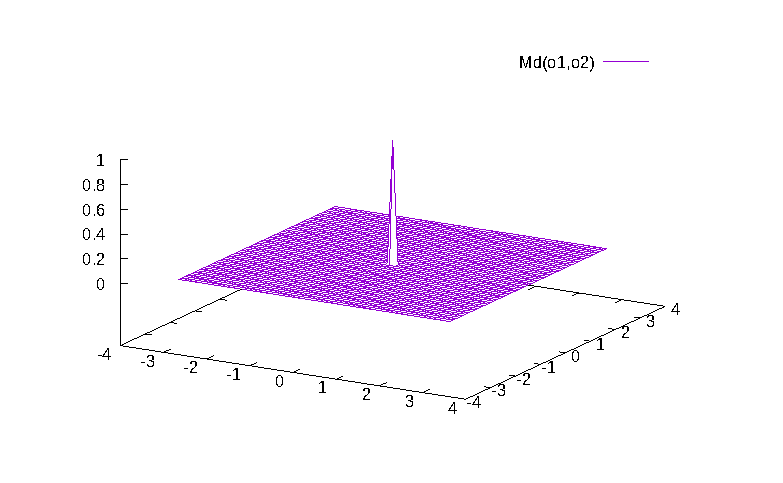
\includegraphics{md}
\end{figure}

\end{document}
